\documentclass[10pt]{book}

%These tell TeX which packages to use.
\usepackage{array,epsfig}
\usepackage{amsmath}
\usepackage{amsfonts}
\usepackage{amssymb}
\usepackage{amsxtra}
\usepackage{amsthm}
\usepackage{mathrsfs}
\usepackage{color}
\usepackage{enumitem}
%\usepackage{mdframed}
\usepackage[most]{tcolorbox}
\usepackage{pgfplots}
\pgfplotsset{compat=1.6}

\pgfplotsset{soldot/.style={color=black,only marks,mark=*}} \pgfplotsset{holdot/.style={color=black,fill=white,only marks,mark=*}}

%Here I define some theorem styles and shortcut commands for symbols I use often
\theoremstyle{definition}
\newtheorem{defn}{Definition}
\newtheorem{thm}{Theorem}
\newtheorem{cor}{Corollary}
\newtheorem*{rmk}{Remark}
\newtheorem{lem}{Lemma}
\newtheorem*{joke}{Joke}
\newtheorem{ex}{Example}
\newtheorem*{soln}{Solution}
\newtheorem{prop}{Proposition}

\newcommand{\lra}{\longrightarrow}
\newcommand{\ra}{\rightarrow}
\newcommand{\surj}{\twoheadrightarrow}
\newcommand{\graph}{\mathrm{graph}}
\newcommand{\bb}[1]{\mathbb{#1}}
\newcommand{\Z}{\bb{Z}}
\newcommand{\Q}{\bb{Q}}
\newcommand{\R}{\bb{R}}
\newcommand{\C}{\bb{C}}
\newcommand{\N}{\bb{N}}
\newcommand{\M}{\mathbf{M}}
\newcommand{\m}{\mathbf{m}}
\newcommand{\MM}{\mathscr{M}}
\newcommand{\HH}{\mathscr{H}}
\newcommand{\Om}{\Omega}
\newcommand{\Ho}{\in\HH(\Om)}
\newcommand{\bd}{\partial}
\newcommand{\del}{\partial}
\newcommand{\bardel}{\overline\partial}
\newcommand{\textdf}[1]{\textbf{\textsf{#1}}\index{#1}}
\newcommand{\img}{\mathrm{img}}
\newcommand{\ip}[2]{\left\langle{#1},{#2}\right\rangle}
\newcommand{\inter}[1]{\mathrm{int}{#1}}
\newcommand{\exter}[1]{\mathrm{ext}{#1}}
\newcommand{\cl}[1]{\mathrm{cl}{#1}}
\newcommand{\ds}{\displaystyle}
\newcommand{\vol}{\mathrm{vol}}
\newcommand{\cnt}{\mathrm{ct}}
\newcommand{\osc}{\mathrm{osc}}
\newcommand{\LL}{\mathbf{L}}
\newcommand{\UU}{\mathbf{U}}
\newcommand{\support}{\mathrm{support}}
\newcommand{\AND}{\;\wedge\;}
\newcommand{\OR}{\;\vee\;}
\newcommand{\Oset}{\varnothing}
\newcommand{\st}{\ni}
\newcommand{\wh}{\widehat}
%Pagination stuff.
\setlength{\topmargin}{-0.75in}
\setlength{\oddsidemargin}{0in}
\setlength{\evensidemargin}{0in}
\setlength{\textheight}{9.in}
\setlength{\textwidth}{6.5in}
\pagestyle{empty}
\begin{document}
\begin{flushleft}
Name:\underline{\hspace{13cm}}Date:\underline{\hspace{2cm}}
\end{flushleft}
\begin{center}
{\Large Math 1041-007 \hspace{0.5cm} Section 2.3: Using Limit Laws}
\end{center}
%\vspace{0.2 cm}

\begin{tcolorbox}
\subsection*{Limit Laws}
Suppose $c$ is a constant AND $\displaystyle\lim_{x\rightarrow a}f(x)$, $\displaystyle\lim_{x\rightarrow a}g(x)$ both exist
\begin{enumerate}
    \item[(1)] $\displaystyle\lim_{x\rightarrow a}\left(f(x)+g(x)\right)=\lim_{x\rightarrow a}f(x)+\lim_{x\rightarrow a}g(x)$
    \item[(2)]$\displaystyle\lim_{x\rightarrow a}\left(f(x)-g(x)\right)=\lim_{x\rightarrow a}f(x)-\lim_{x\rightarrow a}g(x)$
    \item[(3)] $\displaystyle\lim_{x\rightarrow a}cf(x)=c\left(\lim_{x\rightarrow a}f(x)\right)$
    \item[(4)]$\displaystyle\lim_{x\rightarrow a}\left(f(x)g(x)\right)=\lim_{x\rightarrow a}f(x)\cdot\lim_{x\rightarrow a}g(x)$
    \item[(5)]$\displaystyle \lim_{x\rightarrow a}\frac{f(x)}{g(x)}=\frac{\displaystyle\lim_{x\rightarrow a} f(x)}{\displaystyle\lim_{x\rightarrow a}g(x)}$ IF $\displaystyle\lim_{x\rightarrow a}g(x)\neq 0$.
\end{enumerate}
\end{tcolorbox}
\subsection*{Intro. Example: Using a graph}
Use the Limit Laws and the graphs of $f$ and $g$ in the figure to evaluate the following limits, if they exist.
\begin{figure}[h!]
    \centering
    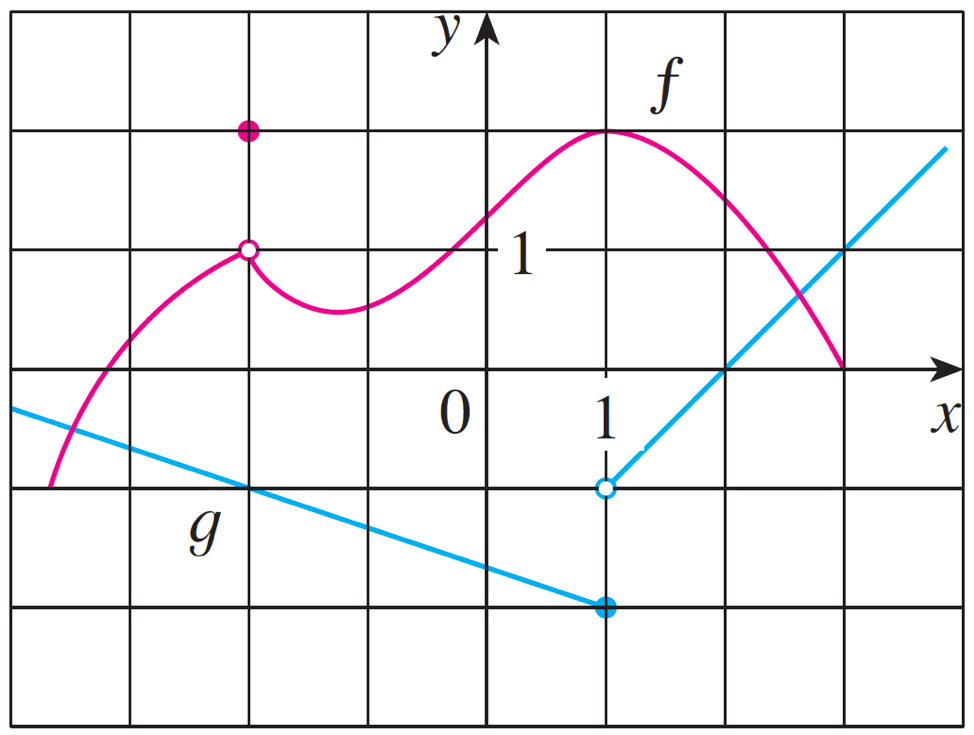
\includegraphics[scale=0.4]{fig1.png}
\end{figure}
\begin{itemize}
\item[(a)]$\displaystyle\lim_{x\rightarrow -2}\left(f(x)+5g(x)\right)$\vspace{2cm}
\item[(b)]$\displaystyle \lim_{x\rightarrow 1}f(x)g(x)$\vspace{2cm}
\item[(c)]$\displaystyle\lim_{x\rightarrow 2}\frac{f(x)}{g(x)}$
\end{itemize}
\clearpage
\begin{tcolorbox}
\subsubsection*{Other Laws!}
\begin{itemize}
    \item $\displaystyle\lim_{x\rightarrow a}\left(f(x)\right)^n=\left(\lim_{x\rightarrow a}f(x)\right)^n$
    \item $\displaystyle\lim_{x\rightarrow a}c=c$, WHY??
    \item $\displaystyle\lim_{x\rightarrow a}x=a$, WHY??
    \item $\displaystyle\lim_{x\rightarrow a}x^n=a^n$ where $n$ is a positive integer.
    \item $\displaystyle\lim_{x\rightarrow a}\sqrt[n]{x}=\sqrt[n]{a}$, NOTE: If $n$ is even then $a>0$, why??
    \item $\displaystyle\lim_{x\rightarrow a}\sqrt[n]{f(x)}=\sqrt[n]{\lim_{x\rightarrow a}f(x)}$, NOTE: If $n$ is even then $\displaystyle\lim_{x\rightarrow a}f(x)>0$, why??
\end{itemize}
\end{tcolorbox}
\subsection*{Example 2: Identify the Laws used in each step}
\begin{align*}
    \lim_{x\rightarrow -2}\frac{x^3+2x^2-1}{5-3x}&=\frac{\displaystyle\lim_{x\rightarrow -2}\left(x^3+2x^2-1\right)}{\displaystyle\lim_{x\rightarrow -2}\left(5-3x\right)}\\[8pt]
    &=\frac{\displaystyle\lim_{x\rightarrow -2}x^3+\lim_{x\rightarrow -2}2x^2-\lim_{x\rightarrow -2}1}{\displaystyle\lim_{x\rightarrow -2}5-\lim_{x\rightarrow -2}3x}
    \\[8pt]
    &=\frac{\displaystyle\lim_{x\rightarrow -2}x^3+2\lim_{x\rightarrow -2}x^2-\lim_{x\rightarrow -2}1}{\displaystyle\lim_{x\rightarrow -2}5-3\lim_{x\rightarrow -2}x}
    \\[8pt]
    &=\frac{(-2)^3+2(-2)^2-1}{5-3(-2)}\\[8pt]
    &=-\frac{1}{11}
\end{align*}
\begin{tcolorbox}
\subsection*{Direct Substitution Property}
If $f$ is a polynomial or a rational function and \underline{$a$ is in the domain of $f$},
\[
\lim_{x\rightarrow a}f(x)=f(a)
\]
\end{tcolorbox}
\subsection*{Example 3: Can we always use Direct Substitution?? (your first limit trick)}
Find $\displaystyle\lim_{x\rightarrow 1}\frac{x^2-1}{x-1}$
\clearpage
\subsection*{Example 4: Piecewise Function} 
Find $\displaystyle\lim_{x\rightarrow 1}g(x)$ where
\[
g(x)=\begin{cases}
x+1 & \textrm{ when }x\neq 1\\
\pi & \textrm{ when }x = 1
\end{cases}
\]
Make a sketch!!
\\ \\ \\ \\ \\ \\ \\ \\ \\ \\ 
\subsection*{Example 5: Find the Limits explain why/why not U can use Substitution!}
\begin{itemize}
\item[(a)] Evaluate $\displaystyle\lim_{h\rightarrow 0}\frac{(3+h)^2-9}{h}$\vspace{3in}
\item[(b)] Evaluate $\displaystyle\lim_{t\rightarrow 0}\frac{\sqrt{t^2+9}-3}{t^2}$
\end{itemize}
\clearpage
\begin{tcolorbox}
\subsubsection*{Your First Theorem!}
$\displaystyle\lim_{x\rightarrow a}f(x)=L$ if and only if
\centering$\displaystyle\lim_{x\rightarrow a^-}f(x)=L=\lim_{x\rightarrow a^+}f(x)$
\end{tcolorbox}
\subsection*{Example 6: Find the limit (if it exists) and explain why/why not it exists!! Make sketches!}
\begin{itemize}
    \item[(a)] $\displaystyle \lim_{x\rightarrow 0}|x|$\vspace{2in}
    \item[(b)] $\displaystyle \lim_{x\rightarrow 0}\frac{|x|}{x}$\vspace{2in}
    \item[(c)] $\displaystyle \lim_{x\rightarrow 4}f(x)$ where
    \[
    f(x)=\begin{cases}
    \sqrt{x-4} & x>4\\
    8-2x & x<4
    \end{cases}
    \]
\end{itemize}
\clearpage
\begin{tcolorbox}
\subsubsection*{The Squeeze Theorem}
If $f(x)\leq g(x)\leq h(x)$ when $x$ is \underline{near} $a$ (except possibly at $a$) and
\[
\lim_{x\rightarrow a}f(x)=\lim_{x\rightarrow a}h(x)=L
\]
then
\[
\lim_{x\rightarrow a}g(x)= L
\]
\end{tcolorbox}
\begin{figure}[h!]
    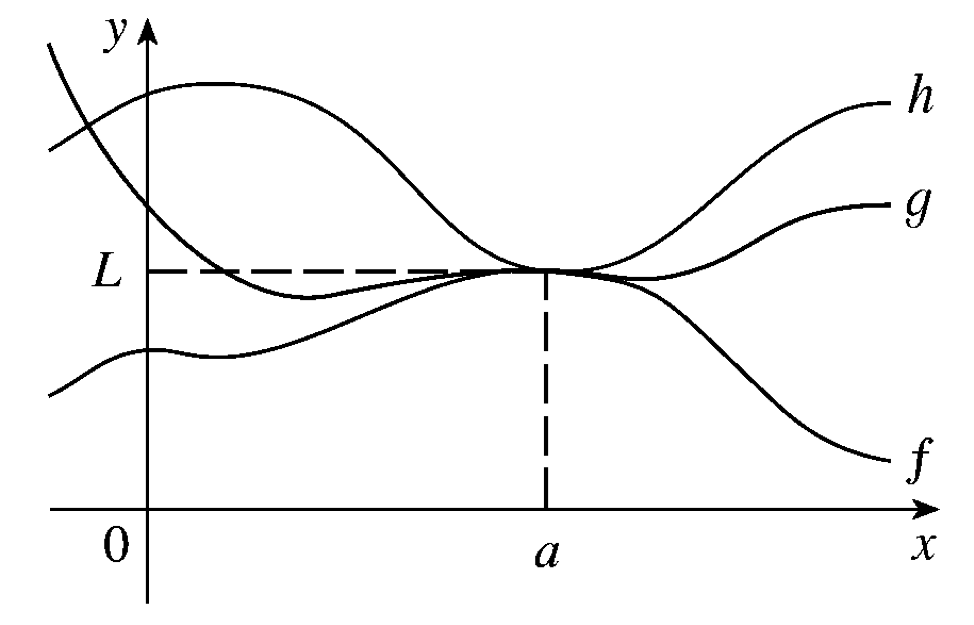
\includegraphics[scale=0.35]{fig2.png}
\end{figure}
\subsubsection*{Example 7: Using Squeeze Theorem}
\begin{itemize}
    \item[(a)] Show that $\displaystyle\lim_{x\rightarrow 0 }x^2\sin\frac{1}{x}=0$\vspace{2in}
    \item[(b)] Find $\displaystyle\lim_{x\rightarrow 0}x^2e^{\sin\frac{1}{x}}$
\end{itemize}
\end{document}